\documentclass[11pt,a4paper]{article}
\usepackage{amsmath}
\usepackage{enumerate}
\usepackage{fancyhdr}
\usepackage{graphicx}
\usepackage[utf8]{inputenc}
\usepackage[a4paper, top=1in, bottom=1.25in, left=0.75in, right=0.75in]{geometry}

\begin{document}
\pagestyle{fancy}
\fancyhead[R]{Niels Hoppe xxxxxx, Robert Schüle xxxxxx, Christoph Ende 331655}

\section{Connectionist Neurons and Multi Layer Perceptrons}

%%%%%%%%%%%%%%%%%%%%%%%%%%%%%%%%%%%%%%%%%%%%%%%%%%%%%%%%%%%%%%%%%%%%%%%%%%%%%%%%
\subsection{Terminology}

\begin{enumerate}[a)]
\item


\end{enumerate}
%%%%%%%%%%%%%%%%%%%%%%%%%%%%%%%%%%%%%%%%%%%%%%%%%%%%%%%%%%%%%%%%%%%%%%%%%%%%%%%%
\subsection{Finding Parameters of a Connectionist Neuron}

\begin{enumerate}[a)]
\item


\end{enumerate}
%%%%%%%%%%%%%%%%%%%%%%%%%%%%%%%%%%%%%%%%%%%%%%%%%%%%%%%%%%%%%%%%%%%%%%%%%%%%%%%%
\subsection{Learning paradigms}

\begin{enumerate}[a)]
\item

\item
\begin{figure}[h]
  \centering
  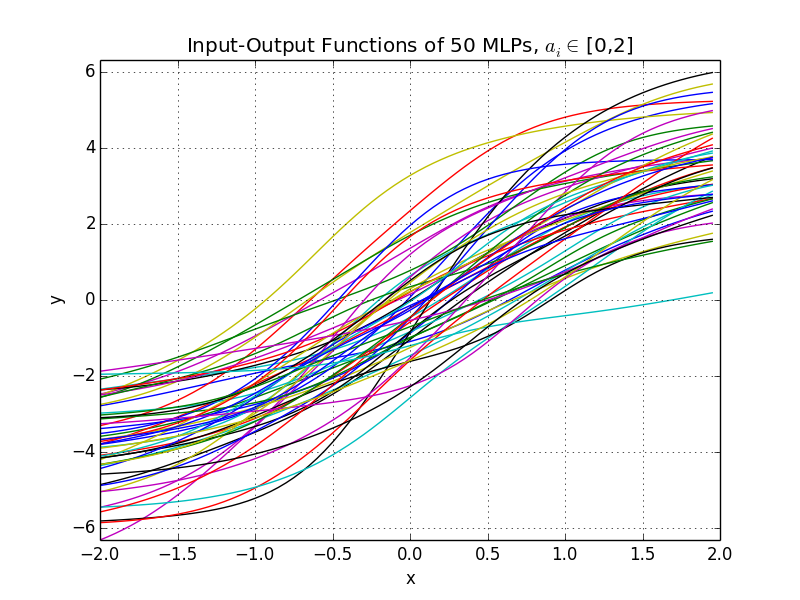
\includegraphics[width=13 cm]{23b.png}
  %\caption{Energy Decay Curve}
  \label{23b}
\end{figure}


\item
\begin{figure}[h]
  \centering
  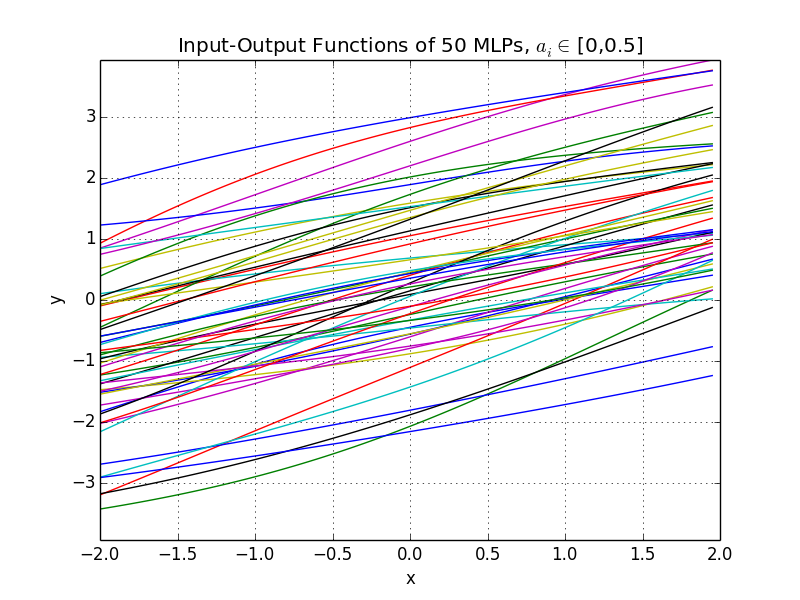
\includegraphics[width=13 cm]{23c.png}
  %\caption{Energy Decay Curve}
  \label{23c}
\end{figure}


\end{enumerate}
%%%%%%%%%%%%%%%%%%%%%%%%%%%%%%%%%%%%%%%%%%%%%%%%%%%%%%%%%%%%%%%%%%%%%%%%%%%%%%%%
\end{document}
